\section{Gestion du projet}

%Ceci est une idée de structure
Cette partie présente une estimation de l'effort en temps pour deux ingénieurs.
Elle se présente sous forme d'un planning définie à l'échelle de la journée.
La figure \ref{fig:planification} illustre l'organisation du travail.
L'axe temporel est horizontal, à droite on retrouve le planning de Bob et à droite celui de Léa, nommés aussi par convention.

\begin{figure}[H]
	\centering
	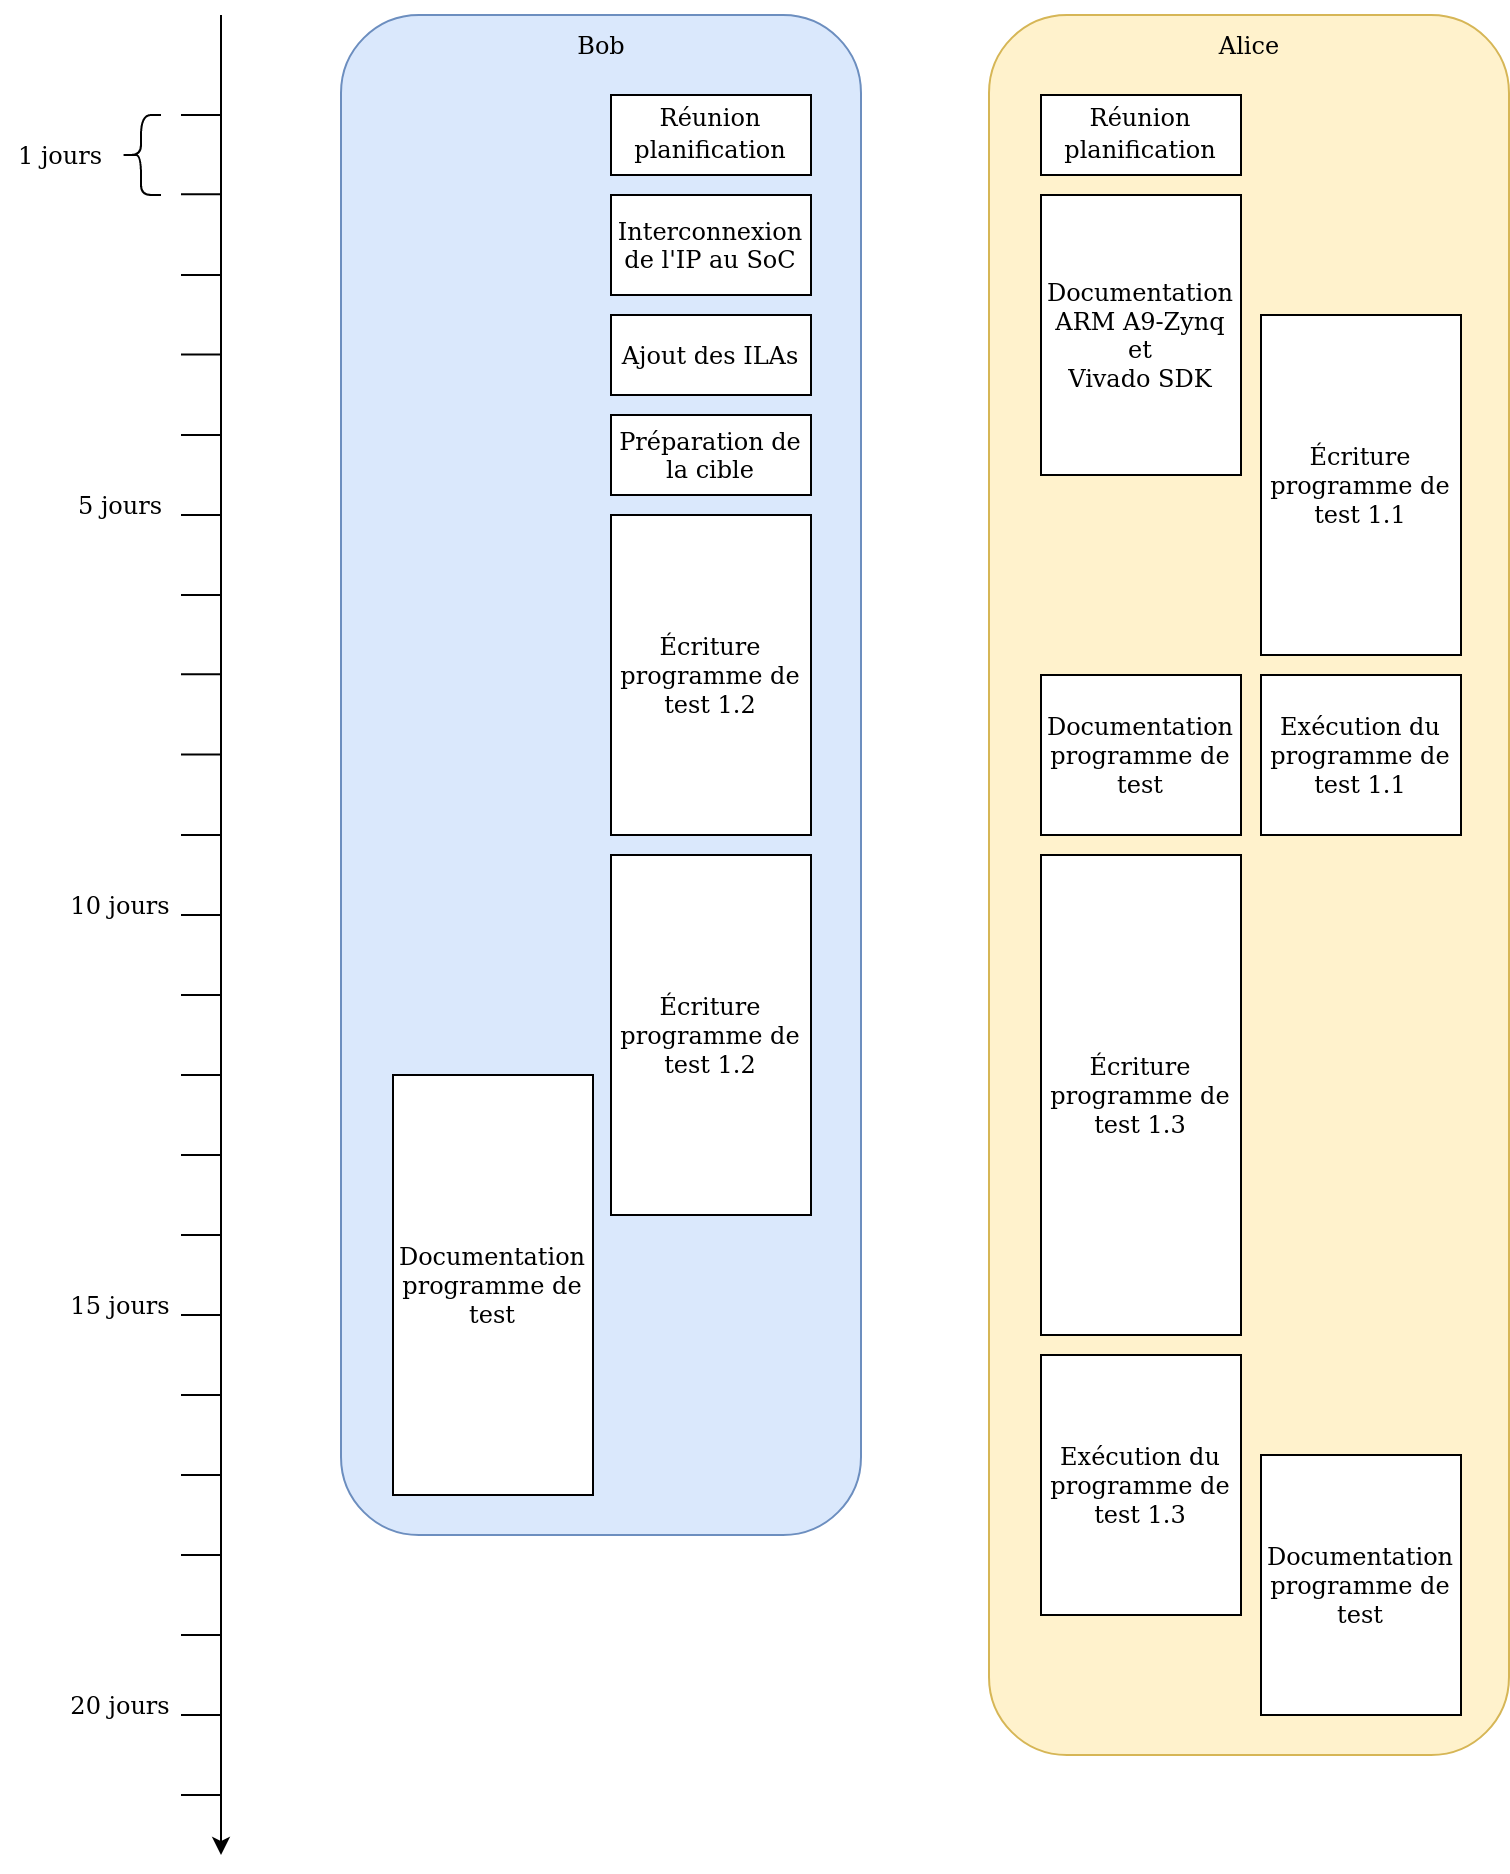
\includegraphics[width=0.75\linewidth]{figure/planning_integration.png}
	\caption{Planification du projet}
	\label{fig:planification}
\end{figure}
La première étape se concentre sur l'organisation et la planification.
Elle comprend une éventuelle communication avec d'autres équipes et une contextualisation du projet.
Après cela, les deux ingénieurs travaillent en parallèle.
Bob se charge de mettre en place l'environnement de développement matériel pendant les 4 premiers jours.
Il devra ajouter l'IP au sein de la plateforme existante en l'interconnectant au bus AXI et aux signaux d'interruptions.
Les blocs ILAs sont ajoutés dès la première synthèse.
La préparation de la cible fait référence à tout ce qui touche à la carte physique et sa bonne connexion au PC de développement.
Pendant ce même temps Alice commence à s'approprier les ressources logicielles et notamment l'implémentation des deux cortex A9 qui, selon nous représente des difficultés importantes.
Elle rédige ensuite, le premier programme de test visant à valider le bon fonctionnement des lectures écritures.
Cette tâche semble plutôt simple, mais nous considérons qu'Alice n'est pas experte de la carte Zynq-7000 et qu'elle doit donc trouver ses marques.
Une fois le développement des programmes de test lancé, les deux ingénieurs devront rédiger la documentation de leur travail en parallèle.
Il est important de garder à l'esprit que le test deux ne peut être exécuté que lorsque le premier est validé. 
Valable aussi pour 3 et 2.
La rédaction des programmes peut elle commencer avant la validation du test n-1.
Bien qu'il existe de nombreuses dépendances entre les tâches, cette seconde propriété devrait apporter de la flexibilité au projet.
L'équipe de développement étant constituée de deux membres, le temps de réunion n'a pas été explicitement défini, mais a été intégré directement aux tâches.
Leur communication est essentielle et devra se faire en continu.








\subsection{Risques}

% On fait une petite matrice des risques ? 

% Idées des risques :
%Mauvaise conception de l'IP (bug)
%Couverture de test de simulation d'une IP qui n'est pas complète
%Problème matériel de la cible
%Covid, oh shit here we go again
%Guerre, parce qu'on acceptera jamais les différences de chacun
%Perte d'une ressource (un ingé), c'est horrible
%Outils (Xilinx Vivado,Xilinx SDK) non fonctionnel
%Programme de tests marche pas
%Temps de synthèse négligé

\begin{table}[H]
	\centering
	\begin{tabular}{|p{2cm}|c|c|c|c|}
		\hline
		occurrence \newline gravité &1	& 2 & 3 \\ \hline
		1	&  \cellcolor{green} & B \cellcolor{green} & A \cellcolor{orange} \\ \hline
		2	& \cellcolor{green}	& E \cellcolor{orange}	& \cellcolor{red} \\ \hline
		3	& D \cellcolor{orange}	& C	\cellcolor{red}& \cellcolor{red}\\ \hline
	\end{tabular}
	\hspace{2cm}
	\begin{tabular}{|c|c|}
		\hline
		Label & Risque \\ \hline
		A	\cellcolor{orange} &	Communication \\ \hline
		B	\cellcolor{green} &	Répartition du travail \\ \hline
		C	\cellcolor{red} &	Ré-employabilité \\ \hline
		D	\cellcolor{orange} &	Erreur de modélisation \\ \hline
		E	\cellcolor{orange} &	Risque pandémique \\ \hline
	\end{tabular}
	\caption{Matrice de sévérité et labels correspondants}
\end{table}
